\documentclass[twoside,9pt]{book}
\makeatletter
\@mparswitchtrue
\usepackage{phd}
\usepackage{xhfill}
\newfontfamily{\documentfont}{Arial}[Scale=1.3,Script=Latin]
\baselineskip1.5\baselineskip
\parindent0pt
\begin{document}
\documentfont
\mbox{}

\lineskip0pt
\newlength\topofpage

\setlength{\topofpage}{-1in-\topmargin-\headheight-\headsep-\topskip}

\newlength\leftpagepoint
\setlength{\leftpagepoint}{\oddsidemargin+1in}


\vspace*{\the\topofpage}\vskip0pt %
%\setlength{\topofpage}{-\topofpage}
\noindent\hbox to 0pt{\vrule height -\topofpage width 1pt} \tikz \draw (0,0) -- (-5,-1in);%
\vskip0pt %
\vbox to 0pt {%
   \hbox to 0pt{\llap{\hbox{\rule{\oddsidemargin+1in-5pt}{2pt}}}}%
   \hbox to 0pt{\color{magenta}\rule{\textwidth}{2pt}}%
   \mbox{\color{green}\rule{\marginparwidth}{2pt}}%
   \mbox{\color{red!50}\rule{\marginparsep}{2pt}}%
   \mbox{\color{red!20}\rule{.2in-2pt}{2pt}}%
   %
   \vskip0pt %
   
    
    %
 }%    
\mbox{\rule{2pt}{3cm}}\raisebox{5pt}{\makebox[0pt][l]{\HHUGE 1}}%
   \rule{1.3cm}{2pt}\raisebox{-7pt}{\mbox{\Huge\color{teal}Determinants}}%
   \vskip0pt %
   \raisebox{0cm}[0pt][0cm]{%
   \color{thegray}%
   \hbox to \textwidth{%
        \hfill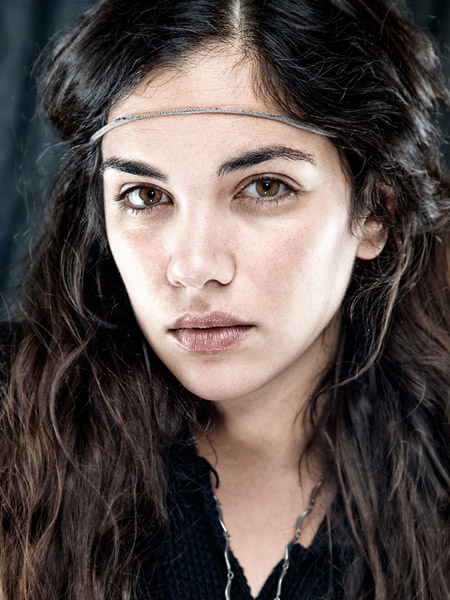
\includegraphics[width=3cm]{./images/amato.jpg}%
        \kern8pt\rule{2.5pt}{4cm}
    }}%
    \vskip0pt %
    % bottom image ru;e
    \hbox to \textwidth{%
        \hfill\hbox{\color{thegray}\rule{3.5cm}{2.5pt}}\kern-3.5pt\rule{2.5pt}{13pt}%
       }
\vskip5cm

\expandafter\the\topofpage\par

\def\fullwidthrule{%
\expandafter\ifodd\thepage%
   \setlength{\leftpagepoint}{\oddsidemargin+1in}%
\else%
   \setlength{\leftpagepoint}{\evensidemargin+1in+\marginparsep}%
\fi%
\bgroup

\lineskip0pt% 
\baselineskip0pt
\parindent0pt%
\parskip0pt%
\leftskip-\leftpagepoint\relax
\leavevmode\noindent%
\hbox{\tikz\draw[color=green, inner sep=0pt,outer sep=0pt, line width=50pt] (0,0) --(\pdfpagewidth,0pt);%
}%
\vskip-2pt
\par%

\hsize=\pdfpagewidth
\@themargin=0pt
\moveleft10pt\vbox{\lorem}
\egroup%
}%

\fullwidthrule

\newpage
   
Testing something\par    
\fullwidthrule   

   

\oddsidemargin=2cm
\hoffset=-1in
%\textwidth=\pdfpagewidth
  
  ..\par
  
\lorem%

\cxset{geometry units=pc,
          geometry lines color=red,
          geometry grid color=white,
          geometry diagonal=false}
          
\pagestyle{grid}

\newpage

\lipsum

\printreadability

\end{document}